
\documentclass[journal]{IEEEtran}
\usepackage[utf8]{inputenc}
\usepackage{graphicx}
\usepackage{subfig}
\usepackage{amsmath}
\usepackage{multicol}
\usepackage{ragged2e}
\usepackage{siunitx}
\usepackage{tikz}
\usepackage{tikz-3dplot}
\usetikzlibrary{shapes,arrows}
\usepackage{pgfplots}
\pgfplotsset{compat=newest}
\pgfplotsset{plot coordinates/math parser=false}
\newlength\figureheight
\newlength\figurewidth
\renewcommand\labelitemi{--}

\usepackage{ifthen}
\usepackage{ifpdf}
\ifpdf
\usepackage[pdftex]{hyperref}
\else
\usepackage{hyperref}
\fi
\usepackage{color}


\begin{document}

\title{Space Exploration Engineering\\
Mid-term Report A2}

\author{Romain~Pessia — Student Number 81723435 \\
Fall 2017, Keio University }%

\maketitle

\section*{Introduction}

The purpose of this assignment is to put into practice the Clohessy–Wiltshire equations with a simple rendez-vous case between a target and a chaser without means of propulsion. Namely, we will first study how to find the appropriate initial velocity of the chaser, given a desired configuration at a certain time $T$; then, we will look into the velocity at the time of rendez-vous as well as the overall trajectory of the spacecraft.

\section*{A2a: two-impulse rendez-vous maneuver}

In this section, we consider a target---on a circular orbit around the Earth---and a chaser, whose coordinates are defined on a target-centered, target-fixed frame of reference. As such, we define the coordinates of the chaser in this frame of reference wrt. a certain time $t$ as

\begin{equation}
    \vec{X}(t) = \begin{bmatrix} x(t)\\
    y(t)\\
    z(t)\end{bmatrix}
\end{equation}

The velocity of the chaser is thus defined as follows:

\begin{equation}
    \vec{V}(t) = \begin{bmatrix} \dot{x}(t)\\
    \dot{y}(t)\\
    \dot{y}(t)\end{bmatrix}
\end{equation}

The Clohessy–Wiltshire equations, applied to the system considered, can then be written under the form

\begin{equation}
\label{cw}
    \begin{bmatrix}
    \vec{X}(t)\\
    \vec{V}(t)\\
    \end{bmatrix}
    =
    \begin{bmatrix}
    A(t) & B(t)\\
    C(t) & D(t)\\
    \end{bmatrix}
    \begin{bmatrix}
    \vec{X}(0)\\
    \vec{V}(0)\\
    \end{bmatrix}
\end{equation}

Where

\begin{equation*}
    A(t)= \begin{bmatrix}
    1 & 0 & 6(s\theta-\theta)\\
    0 & c \theta & 0 \\
    0 & 0 & 4-3c\theta
    \end{bmatrix}
\end{equation*}
\begin{equation*}    
    B(t)= \begin{bmatrix}
    (4/\omega)s\theta-3t & 0 & (2/\omega)(c\theta-1) \\
    0 & (1/\omega)s\theta & 0 \\
    (2/\omega)(1-c\theta) & 0 & (1/\omega)s\theta
    \end{bmatrix}
\end{equation*}
\begin{equation*}    
    C(t) =  \begin{bmatrix}
    0 & 0 & 6\omega(c\theta-1) \\
    0 & -\omega s\theta & 0 \\
    0 & 0 & 3\omega s\theta \end{bmatrix}
\end{equation*}
\begin{equation*}    
    D(t) =  \begin{bmatrix}
    4c\theta-3 & 0 & -2s\theta \\
    0 & c\theta & 0 \\
    2s\theta & 0 & c\theta \end{bmatrix}
\end{equation*}
With $\omega$ the angular speed of the target in its circular rotation around the Earth, and $\theta$ defined as being equal to $\omega t$. Additionally, $c\theta$ and $s\theta$ stand for $\cos{\theta}$ and $\sin{\theta}$ respectively.

A consequence of Equation \ref{cw} is:

\begin{equation}
\label{cw2}
\forall t\geq 0, \vec{X}(t)=A(t)\vec{X}(0)+B(t)\vec{V}(0) 
\end{equation}

Let us now consider a hypothetical time $T$ where the chaser meets the target. In other terms,

\begin{equation}
    \vec{X}(T) = \vec{0}
\end{equation}

Using Equation \ref{cw2}, we derive the following:

\begin{equation}
    A(T)\vec{X}(0)+B(T)\vec{V}(0)=\vec{0}
\end{equation}
\begin{equation}
    \vec{V}(0)=-B^{-1}(T)A(T)\vec{X}(0) 
\end{equation}
The above formula is valid as long as B is invertible, which requires that $8(1-\cos{(\omega T)}) - 3 \omega T \sin{(\omega T)} \neq 0$


Similarly, we can calculate the velocity of the chaser at the time $T$ thanks to the formula:
\begin{equation}
    \vec{V}(T)=C(T)\vec{X}(0)+D(T)\vec{V}(0) 
\end{equation}

\section*{A2b: study of the trajectory}

In order to study the trajectory of the chaser wrt. the target, we developed a program in C++ which calculates the coordinates of the chaser until contact, given initial information on the problem. The source code for the program can be found on \cite{git_program}.

First, let us consider a simple case such as the one proposed for the assignment, and described by the table below.

\begin{table}[h!]
\centering
 \begin{tabular}{| c | c |} 
 \hline
 $x_0$ & 100 \si{km}\\
 $y_0$ & 0 \si{m}\\
 $z_0$ & 0 \si{m}\\
 $h$ & 400 \si{km} \\
 $T$ & 3600 \si{s}\\
 \hline
\end{tabular}
\caption{Parameters for the first test}
\end{table}

Given these initial conditions, the program computes all positions of the chaser until the time of rendez-vous. Figure \ref{plot:xz} shows the trajectory followed by the spacecraft, only considering its $x$ and $z$ coordinates ($y$ stays equal to zero for the whole trajectory because of the initial position of the chaser).
    \begin{figure}[htp!]
      \centering
      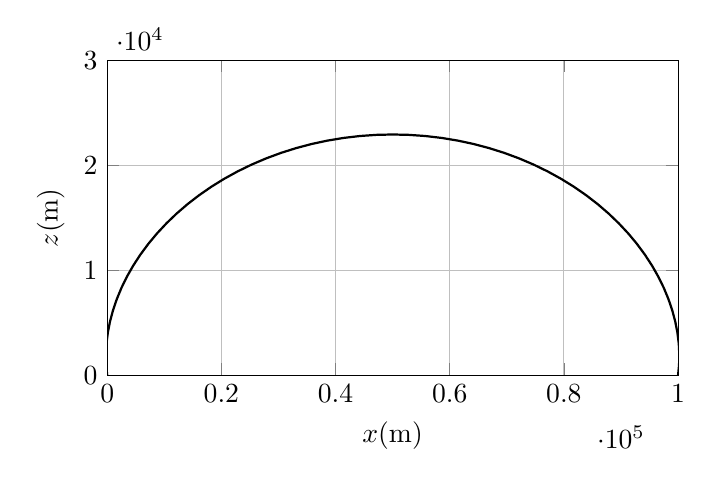
\begin{tikzpicture}

\begin{axis}[%
view={0}{90},
width=7.25cm,
height=4cm,
scale only axis,
xmin=0, xmax=100000,
xlabel={$x$(m)},
xmajorgrids,
ymin=0, ymax=30000,
ylabel=$z$(m),
ymajorgrids,
legend cell align=left,
legend pos = south east,
legend style={align=left}]
\addplot [
color=black,
thick,
mark=none,
mark options={solid}
]
coordinates{
(100000,0)(100177,973.387)(100219,1975.25)(100124,3000.95)(99887.2,4045.75)(99507.7,5104.83)(98983.6,6173.29)(98313.8,7246.19)(97498.1,8318.58)(96536.8,9385.5)(95431.2,10442)(94182.8,11483.3)(92794.2,12504.4)(91268.4,13500.7)(89609,14467.7)(87820.5,15400.7)(85907.6,16295.6)(83875.8,17148.1)(81731.2,17954.3)(79480.4,18710.6)(77130.3,19413.3)(74688.4,20059.4)(72162.8,20645.7)(69561.6,21169.6)(66893.6,21628.6)(64167.7,22020.7)(61393.1,22343.9)(58579.4,22596.9)(55736.1,22778.5)(52873,22887.8)(50000,22924.2)(47127,22887.8)(44263.9,22778.5)(41420.6,22596.9)(38606.9,22343.9)(35832.3,22020.7)(33106.4,21628.6)(30438.4,21169.6)(27837.2,20645.7)(25311.6,20059.4)(22869.7,19413.3)(20519.6,18710.6)(18268.8,17954.3)(16124.2,17148.1)(14092.4,16295.6)(12179.5,15400.7)(10391,14467.7)(8731.59,13500.7)(7205.76,12504.4)(5817.15,11483.3)(4568.82,10442)(3463.17,9385.5)(2501.94,8318.58)(1686.22,7246.19)(1016.41,6173.29)(492.253,5104.83)(112.798,4045.75)(-123.561,3000.95)(-219.093,1975.25)(-176.72,973.387)(0,0)

};
\end{axis}
\end{tikzpicture}%
      \caption{Trajectory of the chaser from $t=0$ to $t=T$}
      \label{plot:xz}
    \end{figure}

\begin{figure}[htp!]
  \centering
  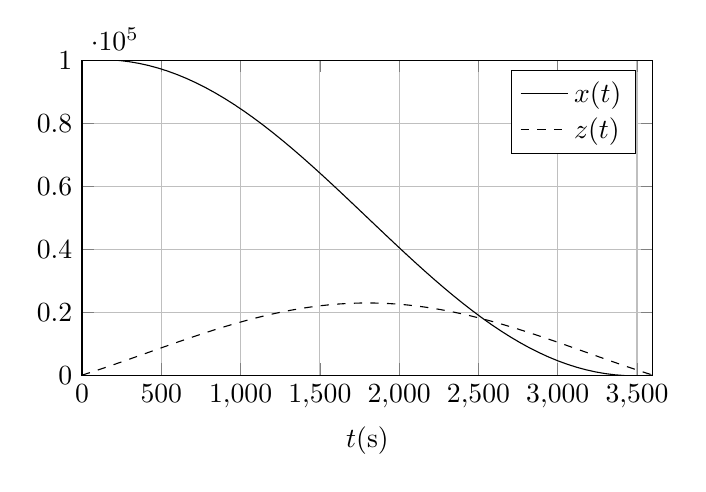
\begin{tikzpicture}

\begin{axis}[%
view={0}{90},
width=7.25cm,
height=4cm,
scale only axis,
xmin=0, xmax=3600,
xlabel={$t$(s)},
xmajorgrids,
ymin=0, ymax=100000,
ymajorgrids,
legend cell align=left,
legend pos = north east,
legend style={align=left}]
\addplot [
color=black,
solid,
mark options={solid}
]
coordinates{
(0,100000)(60,100177)(120,100219)(180,100124)(240,99887.2)(300,99507.7)(360,98983.6)(420,98313.8)(480,97498.1)(540,96536.8)(600,95431.2)(660,94182.8)(720,92794.2)(780,91268.4)(840,89609)(900,87820.5)(960,85907.6)(1020,83875.8)(1080,81731.2)(1140,79480.4)(1200,77130.3)(1260,74688.4)(1320,72162.8)(1380,69561.6)(1440,66893.6)(1500,64167.7)(1560,61393.1)(1620,58579.4)(1680,55736.1)(1740,52873)(1800,50000)(1860,47127)(1920,44263.9)(1980,41420.6)(2040,38606.9)(2100,35832.3)(2160,33106.4)(2220,30438.4)(2280,27837.2)(2340,25311.6)(2400,22869.7)(2460,20519.6)(2520,18268.8)(2580,16124.2)(2640,14092.4)(2700,12179.5)(2760,10391)(2820,8731.59)(2880,7205.76)(2940,5817.15)(3000,4568.82)(3060,3463.17)(3120,2501.94)(3180,1686.22)(3240,1016.41)(3300,492.253)(3360,112.798)(3420,-123.561)(3480,-219.093)(3540,-176.72)(3600,0)
};
\addlegendentry{$x(t)$};

\addplot [
color=black,
dashed,
mark options={solid}
]
coordinates{
(0,0)(60,973.387)(120,1975.25)(180,3000.95)(240,4045.75)(300,5104.83)(360,6173.29)(420,7246.19)(480,8318.58)(540,9385.5)(600,10442)(660,11483.3)(720,12504.4)(780,13500.7)(840,14467.7)(900,15400.7)(960,16295.6)(1020,17148.1)(1080,17954.3)(1140,18710.6)(1200,19413.3)(1260,20059.4)(1320,20645.7)(1380,21169.6)(1440,21628.6)(1500,22020.7)(1560,22343.9)(1620,22596.9)(1680,22778.5)(1740,22887.8)(1800,22924.2)(1860,22887.8)(1920,22778.5)(1980,22596.9)(2040,22343.9)(2100,22020.7)(2160,21628.6)(2220,21169.6)(2280,20645.7)(2340,20059.4)(2400,19413.3)(2460,18710.6)(2520,17954.3)(2580,17148.1)(2640,16295.6)(2700,15400.7)(2760,14467.7)(2820,13500.7)(2880,12504.4)(2940,11483.3)(3000,10442)(3060,9385.5)(3120,8318.58)(3180,7246.19)(3240,6173.29)(3300,5104.83)(3360,4045.75)(3420,3000.95)(3480,1975.25)(3540,973.387)(3600,0)
};
\addlegendentry{$z(t)$};
\end{axis}
\end{tikzpicture}%
  \caption{$x$ and $z$ coordinates of the chaser as a function of time}
  \label{plot:xzt}
\end{figure}
This ellipse-shaped trajectory is coherent with the model used and the case studied where only $x_0$ is not equal to zero. We can also draw the evolution of both $x$ and $z$ coordinates as a function of time, as can be seen in Figure \ref{plot:xzt}.



Both figures show evidence that the target does meet the chaser at $t=T$, as predicted by the equations.

The program also works for non-zero values of $y_0$ and $z_0$, as the plots in Figure \ref{plot:3d} and Figure \ref{plot:xyz} showcase.

\begin{table}[h!]
\centering
 \begin{tabular}{| c | c |} 
 \hline
 $x_0$ & 100 \si{km}\\
 $y_0$ & 100 \si{km}\\
 $z_0$ & 100 \si{km}\\
 $h$ & 400 \si{km} \\
 $T$ & 3600 \si{s}\\
 \hline
\end{tabular}
\caption{Parameters for the second test}
\end{table}

\begin{figure}[htp!]
  \centering
  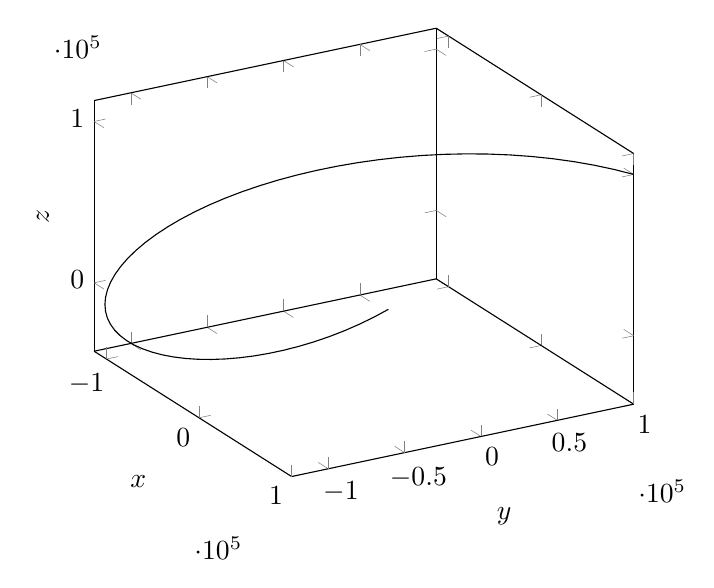
\begin{tikzpicture}
\begin{axis}
    [
    view={60}{30},
    xlabel = {$x$},
    ylabel = {$y$},
    zlabel={$z$}
    ]
\addplot3[
    samples = 60,
]coordinates{(100000,100000,100000)(87626.1,94784,99600.5)(75326.8,89130,98903.9)(63142.2,83064.1,97913.4)(51112,76614.5,96633.6)(39275.2,69810.8,95070.4)(27669.8,62684.5,93231.1)(16332.8,55268.6,91124.1)(5300.03,47597.3,88759.2)(-5394.28,39706.1,86147.3)(-15717.3,31631.4,83300.5)(-25638,23410.5,80231.9)(-35127.2,15081.5,76955.6)(-44157.6,6682.78,73487)(-52704.1,-1746.83,69841.9)(-60743.9,-10168.4,66037.2)(-68256.6,-18542.9,62090.5)(-75223.9,-26831.8,58020.1)(-81630.4,-34996.7,53844.7)(-87463.1,-42999.8,49583.6)(-92711.7,-50804.3,45256.5)(-97368.5,-58374,40883.5)(-101429,-65674,36484.7)(-104890,-72670.6,32080.4)(-107753,-79331.3,27691.1)(-110022,-85625.5,23336.9)(-111702,-91524,19038)(-112803,-96999.6,14814.3)(-113335,-102027,10685.3)(-113313,-106583,6670.03)(-112755,-110646,2787.09)(-111678,-114199,-945.596)(-110105,-117223,-4510.77)(-108059,-119706,-7891.96)(-105567,-121636,-11073.6)(-102657,-123003,-14040.8)(-99358.4,-123802,-16780.1)(-95703.8,-124030,-19278.7)(-91726.5,-123684,-21525.1)(-87461.5,-122766,-23508.8)(-82945,-121282,-25220.8)(-78214.8,-119237,-26653.2)(-73309.1,-116641,-27799.2)(-68267.4,-113505,-28653.6)(-63129.6,-109846,-29212.5)(-57936,-105679,-29473.3)(-52727.3,-101023,-29434.8)(-47544.1,-95901.3,-29097.1)(-42427.2,-90335.9,-28461.8)(-37416.7,-84353.2,-27531.9)(-32552.5,-77980.6,-26311.6)(-27873.6,-71247.7,-24806.5)(-23418.4,-64185.7,-23023.8)(-19224,-56827,-20971.5)(-15326.4,-49205.7,-18659.1)(-11760.4,-41357.1,-16097.4)(-8559.01,-33317.3,-13298.2)(-5753.66,-25123.7,-10274.4)(-3373.97,-16813.9,-7039.99)(-1447.57,-8426.41,-3609.9)(0,0,0)
};
\end{axis}
\end{tikzpicture}
  \caption{3D trajectory of the chaser from $t=0$ to $t=T$}
  \label{plot:3d}
\end{figure}

\begin{figure}[htp!]
  \centering
  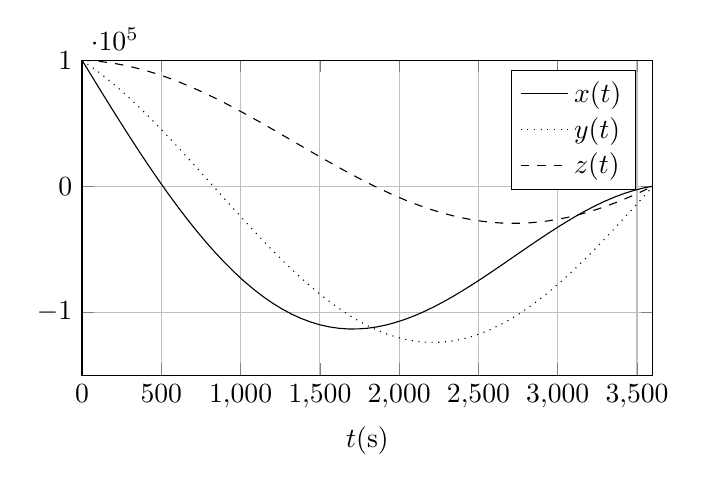
\begin{tikzpicture}

\begin{axis}[%
view={0}{90},
width=7.25cm,
height=4cm,
scale only axis,
xmin=0, xmax=3600,
xlabel={$t$(s)},
xmajorgrids,
ymin=-150000, ymax=100000,
ymajorgrids,
legend cell align=left,
legend pos = north east,
legend style={align=left}]
\addplot [
color=black,
solid,
mark options={solid}
]
coordinates{
(0,100000)(60,87626.1)(120,75326.8)(180,63142.2)(240,51112)(300,39275.2)(360,27669.8)(420,16332.8)(480,5300.03)(540,-5394.28)(600,-15717.3)(660,-25638)(720,-35127.2)(780,-44157.6)(840,-52704.1)(900,-60743.9)(960,-68256.6)(1020,-75223.9)(1080,-81630.4)(1140,-87463.1)(1200,-92711.7)(1260,-97368.5)(1320,-101429)(1380,-104890)(1440,-107753)(1500,-110022)(1560,-111702)(1620,-112803)(1680,-113335)(1740,-113313)(1800,-112755)(1860,-111678)(1920,-110105)(1980,-108059)(2040,-105567)(2100,-102657)(2160,-99358.4)(2220,-95703.8)(2280,-91726.5)(2340,-87461.5)(2400,-82945)(2460,-78214.8)(2520,-73309.1)(2580,-68267.4)(2640,-63129.6)(2700,-57936)(2760,-52727.3)(2820,-47544.1)(2880,-42427.2)(2940,-37416.7)(3000,-32552.5)(3060,-27873.6)(3120,-23418.4)(3180,-19224)(3240,-15326.4)(3300,-11760.4)(3360,-8559.01)(3420,-5753.66)(3480,-3373.97)(3540,-1447.57)(3600,0)
};
\addlegendentry{$x(t)$};

\addplot [
color=black,
dotted,
mark options={solid}
]
coordinates{
(0,100000)(60,94784)(120,89130)(180,83064.1)(240,76614.5)(300,69810.8)(360,62684.5)(420,55268.6)(480,47597.3)(540,39706.1)(600,31631.4)(660,23410.5)(720,15081.5)(780,6682.78)(840,-1746.83)(900,-10168.4)(960,-18542.9)(1020,-26831.8)(1080,-34996.7)(1140,-42999.8)(1200,-50804.3)(1260,-58374)(1320,-65674)(1380,-72670.6)(1440,-79331.3)(1500,-85625.5)(1560,-91524)(1620,-96999.6)(1680,-102027)(1740,-106583)(1800,-110646)(1860,-114199)(1920,-117223)(1980,-119706)(2040,-121636)(2100,-123003)(2160,-123802)(2220,-124030)(2280,-123684)(2340,-122766)(2400,-121282)(2460,-119237)(2520,-116641)(2580,-113505)(2640,-109846)(2700,-105679)(2760,-101023)(2820,-95901.3)(2880,-90335.9)(2940,-84353.2)(3000,-77980.6)(3060,-71247.7)(3120,-64185.7)(3180,-56827)(3240,-49205.7)(3300,-41357.1)(3360,-33317.3)(3420,-25123.7)(3480,-16813.9)(3540,-8426.41)(3600,0)
};
\addlegendentry{$y(t)$};

\addplot [
color=black,
dashed,
mark options={solid}
]
coordinates{
(0,100000)(60,99600.5)(120,98903.9)(180,97913.4)(240,96633.6)(300,95070.4)(360,93231.1)(420,91124.1)(480,88759.2)(540,86147.3)(600,83300.5)(660,80231.9)(720,76955.6)(780,73487)(840,69841.9)(900,66037.2)(960,62090.5)(1020,58020.1)(1080,53844.7)(1140,49583.6)(1200,45256.5)(1260,40883.5)(1320,36484.7)(1380,32080.4)(1440,27691.1)(1500,23336.9)(1560,19038)(1620,14814.3)(1680,10685.3)(1740,6670.03)(1800,2787.09)(1860,-945.596)(1920,-4510.77)(1980,-7891.96)(2040,-11073.6)(2100,-14040.8)(2160,-16780.1)(2220,-19278.7)(2280,-21525.1)(2340,-23508.8)(2400,-25220.8)(2460,-26653.2)(2520,-27799.2)(2580,-28653.6)(2640,-29212.5)(2700,-29473.3)(2760,-29434.8)(2820,-29097.1)(2880,-28461.8)(2940,-27531.9)(3000,-26311.6)(3060,-24806.5)(3120,-23023.8)(3180,-20971.5)(3240,-18659.1)(3300,-16097.4)(3360,-13298.2)(3420,-10274.4)(3480,-7039.99)(3540,-3609.9)(3600,0)
};
\addlegendentry{$z(t)$};
\end{axis}
\end{tikzpicture}%
  \caption{$x$, $y$ and $z$ coordinates of the chaser as a function of time}
  \label{plot:xyz}
\end{figure}

\appendices

\begin{thebibliography}{9}
\bibitem{git_program} 
Romain Pessia. 
\textit{Two-impulse rendez-vous maneuver calculator}. 
Github project on \href{https://github.com/romainpessia/two-impulse-rendez-vous-maneuver-calculator}{https://github.com/romainpessia/two-impulse-rendez-vous-maneuver-calculator}, 2017.
\end{thebibliography}

\end{document}


